%! TEX root = ../main.tex
\section{Encuesta de Ubicación}
\label{sec:res_ubicacion}

Como se indicó en la sección~\ref{sec:ubicacion}, se agrupa a los alumnos
encuestados de acuerdo a las características de sus dispositivos móviles y del
acceso a internet.

El acceso a internet es un requisito importante, pues para que los mismos puedan
enviar su progreso y así se registre la utilización de la solución, así, es
necesario que los usuarios tengan un acceso ocasional a internet. 

En la figura~\ref{fig:ubicacion_acceso_internet} se puede observar que de 93
encuestados, el $94,6\%$ tiene acceso a internet al menos en algún momento y que
solo el $5.4\%$ no tiene acceso a internet en sus dispositivos móviles, esto
permite que tengan acceso a la solución el $94,6\%$ de los alumnos.

\begin{figure}[H]
\centering
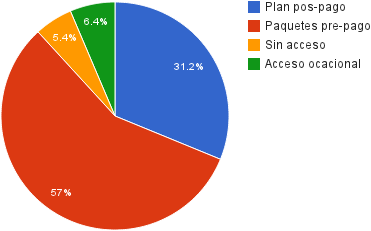
\includegraphics[scale=0.5]{resultados/imagenes/ubicacion_acceso_internet.png}
\caption{Acceso a internet desde dispositivos móviles}
\label{fig:ubicacion_acceso_internet}
\end{figure}

La utilización en dispositivos móviles es un requisito necesario para la
solución, en la figura\ref{fig:ubicacion_sistemas_operativos} se muestra
los sistemas operativos móviles utilizados por los usuarios encuestados, si bien
la herramienta utilizada permite generar clientes a diversos, es importante
conocer el sistema operativo que poseen los alumnos para realizar pruebas.

En la figura~\ref{fig:ubicacion_sistemas_operativos} se puede observar que
\emph{Android} lidera con un $61.3\%$, le sigue Windows Phone con un $12.9\%$.
Si bien, según la tabla~\ref{tab:comparacion_motores_juegos}, \emph{Unity3D}
soporta la mayoría de los sistemas operativos, aún es importante hacer pruebas
sobre un sistema operativo especifico, así se selecciona \emph{Android} por ser
el sistema operativo con mayor cuota entre los alumnos.

\begin{figure}[H]
\centering
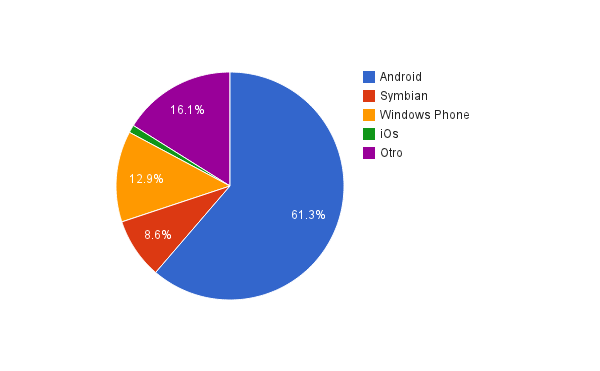
\includegraphics[scale=0.5]{resultados/imagenes/ubicacion_sistemas_operativos.png}
\caption{Sistemas operativos móviles utilizados}
\label{fig:ubicacion_sistemas_operativos}
\end{figure}

Por último, se discrimina a los encuestados para determinar cuantos de ellos
tiene dispositivos móviles que cumplen los requisitos mínimos para utilizar la
solución propuesta según lo descrito en la sección~\ref{sec:ubicacion}. En la
figura~\ref{fig:ubicacion_requisitos_minimos} se puede observar que el $18,3\%$
de los encuestados cumplen con los requisitos.

\begin{figure}[H]
\centering
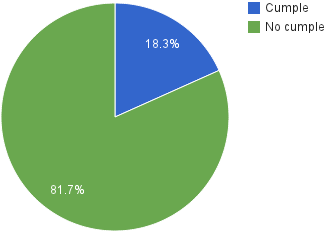
\includegraphics[scale=0.5]{resultados/imagenes/ubicacion_requisitos_minimos.png}
\caption{Dispositivos que cumplen con los requisitos mínimos para la prueba}
\label{fig:ubicacion_requisitos_minimos}
\end{figure}

Si bien los requisitos de la solución no son elevados para los estándares
actuales, la figura~\ref{fig:ubicacion_requisitos_minimos} nos muestra que el
$18.3\%$ tiene dispositivos de alta alta, el cual es un porcentaje mayor al
esperado.

Se observa en la figura~\ref{fig:ubicacion_sistemas_operativos}, que cerca del
$90\%$ posee un dispositivo de gama media o superior, la penetración de los
dispositivos móviles es muy alta en los estudiantes de enfermería.
